\documentclass[conference]{IEEEtran}

\usepackage{epsfig}
\usepackage{url}
\usepackage{cite}
\usepackage{fancybox}
\usepackage{graphicx}
\graphicspath{{images/}}

\begin{document}
\title{Strategies to Combat Administrator Threats to Cloud Computing Systems}
\author{
  \IEEEauthorblockN{Eric Adamski}
  \IEEEauthorblockA{
    School of Computer Science\\
    Carleton University\\
    Ottawa, Ontario, Canada \\
    Email: \{eric.adamski@cmail.carleton.ca\}
  }
  \and
  \IEEEauthorblockN{Shivjot Baidwan}
  \IEEEauthorblockA{
    Ottawa Carleton Institute of Computer Science \\
    University of Ottawa\\
    Ottawa, Ontario, Canada \\
    Email: \{sbaid017@uottawa.ca\}
  }
}

\maketitle

\begin{abstract}
  Cloud services are becoming increasingly popular in the world of technology, as more and more people have come to rely on these services to store personal and private data. Who is to say that the organizations which give cloud based commodities are dependable and secure ? Cloud service providers use techniques such as, data encryption, and cloning for protecting themselves against outside attacks, but individually these techniques lack immunity from the company employees, the insiders. The most essential way which ought to be utilized for protection against threats can be executed at the physical level by having a sturdy infrastructure. It does not do much by itself but it forms the foundation of the strategies to curb the threats, in particular the insider threats. The other strategies which lie atop a solid infrastructure are cloning, encryption, migration, deletion. Throughout the paper we are going to talk about models based on these techniques, how they are applied to conventional computing threats and how this differs from threats to cloud software. This paper will review how modern systems utilize the strategical models previously discussed. In specific we will discuss how these models can be utilized to protect against insider threats.
\end{abstract}

References : TO BE REMOVED \cite{baumann} \cite{subashini} \cite{kamalkant} \cite{chou} \cite{chen} \cite{althebyan} \cite{yun} \cite{sirer} \cite{theoharidou} \cite{bishop} \cite{nguyen} \cite{magklaras} \cite{dimitrios} \cite{suh} \cite{szefer} \cite{oltsik}
\cite{sabahi} \cite{dawoud} \cite{mukherjee} \cite{dwoskin} \cite{spitzner} \cite{kandias}

\IEEEpeerreviewmaketitle

%% Shivu's Stuff %
\section{Introduction}

\textbf{Emerging Trends and Challenges.}
Give a one paragraph overview of the domain that
the paper is going to describe a problem in. Make
sure and reference any existing papers that have
named the domain.

Describe in one paragraph why this domain is important.
It is nice if you can give specific examples of other
research or things that are being done in this domain
that are important to society.

\textbf{Open Problem $\Rightarrow$ Name the problem
you are going to address.}
Now, tell the reader what important problem from
this domain has not been solved that you are going
to attack. Stick to one paragraph. Be VERY specific about what general
problem you are solving.

Briefly discuss and cite in a single paragraph other
research done in this domain. Make sure and explain
why the existing research does not address the
problem that you are describing and solving in the
paper.

If you have some metrics that you are going
to use to claim superiority over prior work, you
can introduce them in a single paragraph here.
Explain why the metrics are important and why
when you evaluate the existing work using these
metrics it motivates your new work.

\textbf{Solution Approach $\Rightarrow$ A pithy
heading for your solution.} To address XYZ
problem, we have done QRS. Describe what you
have done and why it is novel.

In Section~ we present empirical
data that we have gathered from experiments
showing QRS. Give a 1-paragraph overview of
what experiments you ran and how they showed
you were superior to existing solutions.

This paper provides the following contributions
to the study of XYZ:

\begin{itemize}

\item Pithy sentence describing contribution.

\item Pithy sentence describing contribution 2.

\item Pithy sentence describing contribution 3.

\item We present empirical results that show QRS.

\end{itemize}

% Make sure and update this!
%
The remainder of this paper is organized as follows:
Section~\ref{problem_defenition} describes PQR, which we
use as a motivating example throughout the paper;
Section~\ref{background} discusses the challenges that
we faced when ..... ; Section~\ref{solution} covers the our solution to XYZ; Section~ presents empirical
results from analyzing TUV; and Section~\ref{conclusion}
presents concluding remarks and lessons learned.

% Update the heading to match your theme
\section{Problem Defenition}
\label{problem_defenition}

Begin the section with a one paragraph overview
of the section. Outline what the challenges are that
you are going to discuss. You can start the paragraph
with something like "Although XYZ could solve world
hunger, there are a number of challenges to developing
an XYZ."

\subsection{Challenge 1: Something is Hard, Complex, etc.}
\label{challenge1}

You should start out with a one paragraph description of
the challenge. Make sure that you immediately relate the
challenge back to the theme of the paper. Do not introduce
new terminology that you have not previously defined. Make
sure that your description of the challenge is high-level
and clear.

The second paragraph of the challenge should explain how
the challenge concretely manifests in the motivating example.
The first paragraph generally describes the challenge. This
paragraph is showing a specific example of the challenge in
the context of your motivating example. Be very specific
so that the reader understands all of the details. End
the paragraph with a sentence similar to the following:
% Make sure the ref points to a specific subsection in
% the solution section.
Section~ describes how we address this
challenge by QRS.

\subsection{Challenge 2: Something Else is an Issue}
\label{challenge2}

You should start out with a one paragraph description of
the challenge. Make sure that you immediately relate the
challenge back to the theme of the paper. Do not introduce
new terminology that you have not previously defined. Make
sure that your description of the challenge is high-level
and clear.

The second paragraph of the challenge should explain how
the challenge concretely manifests in the motivating example.
The first paragraph generally describes the challenge. This
paragraph is showing a specific example of the challenge in
the context of your motivating example. Be very specific
so that the reader understands all of the details. End
the paragraph with a sentence similar to the following:
% Make sure the ref points to a specific subsection in
% the solution section.
Section~ describes how we address this
challenge by QRS.

\subsection{Challenge 3: Another Painful Issue}
\label{challenge3}

You should start out with a one paragraph description of
the challenge. Make sure that you immediately relate the
challenge back to the theme of the paper. Do not introduce
new terminology that you have not previously defined. Make
sure that your description of the challenge is high-level
and clear.

The second paragraph of the challenge should explain how
the challenge concretely manifests in the motivating example.
The first paragraph generally describes the challenge. This
paragraph is showing a specific example of the challenge in
the context of your motivating example. Be very specific
so that the reader understands all of the details. End
the paragraph with a sentence similar to the following:
% Make sure the ref points to a specific subsection in
% the solution section.
Section~ describes how we address this
challenge by QRS.

\section{Background}
\label{background}

Basically there are three essential service models with respect to the Cloud computing,
specifically (see figure~\ref{services_figure})\footnote{\url{http://cloudprivado.org/wp-content/uploads/2013/04/Cloud-Computing-Saas-Paas-Iaas.jpg}},

\begin{figure}
  \centering
    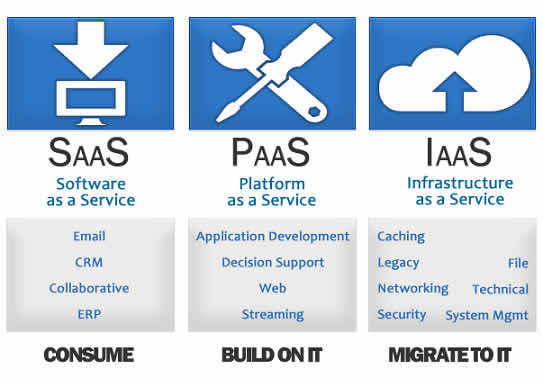
\includegraphics[height=3.5cm, width=4cm]{services}
  \caption{A break down of the main service models.}
  \label{services_figure}
\end{figure}

\subsection{Software as a Service}
Software as a service (SaaS), in which a third party service provider provides the
software.
Cloud application administrations, or Software as a Service (SaaS), portray the biggest
cloud showcase and is evolving rapidly even now. SaaS utilizes the web to convey
applications that are controlled by an outsider seller and whose interface is accessed to
on the customers' side. Most SaaS applications can be run straightforwardly from a web
program with no downloads or installations required, albeit some need the plugins.
On account of the model of web delivery, SaaS eradicates the need to install and run
applications on individual PCs. With SaaS, its simple for business corporations to
streamline their support, on the grounds that everything can be taken care of by the
vendors: applications, runtime, information, middleware, OSes, virtualization, servers,
stockpiling and systems administration.
\subsection{Platform as a Service}
Platform as a service (PaaS), which provides the evolution of newer applications utilizing
the APIs deployed and arranged distantly.
Cloud stage administrations, or Platform as a Service (PaaS), are utilized for applications,
and other innovations, while giving cloud segments to the software. What engineers
pick up with PaaS is a system they can expand upon to create or redo applications. PaaS
makes the testing, improvement, and arrangement of utilizations speedy, basic, and
financially savvy. With this innovation, endeavour operations, or an external supplier,
can oversee OSes, organizing, virtualization, servers, stockpiling, and the PaaS
programming itself. Engineers, on the other hand, deal with the applications.
Undertaking PaaS gives line-of-business programming engineers an organization toward
oneself gateway for overseeing registering framework from brought together IT
operations and the stages that are introduced on top of the equipment. The
undertaking PaaS can be conveyed via a hybrid model that uses both open IaaS and on-
reason framework or as an unadulterated private PaaS that just uses the last.
\subsection{Infrastructure as a Service}
Infrastructure as a service (IaaS), which imparts hardware equipment and the
capabilities of operating systems predominantly through virtualization. Cloud
infrastructure administrations, referred to as Infrastructure as a Service (IaaS), are
organization toward oneself models for getting to, checking, and overseeing remote
datacenter frameworks, for example, register (virtualized or exposed mental),
stockpiling, systems administration (e.g. firewalls). As opposed to needing to buy
equipment out and out, clients can buy IaaS in view of utilization, like power or other
utility charging.
Contrasted with SaaS and PaaS, IaaS clients are in charge of overseeing applications,
information, runtime, middleware, and OSes. Suppliers still oversee virtualization,
servers, hard drives, stockpiling, and systems administration. Numerous IaaS suppliers
now offer databases, informing lines, and different administrations over the
virtualization layer too. Some tech investigators draw a qualification here and utilize the
IaaS+ moniker for these different alternatives. What clients pick up with IaaS is
framework on top of which they can introduce any obliged stage. Clients are in charge
of overhauling these if new forms are discharged.

%%===============%
%% Eric's Stuff  %
\section{Combative Strategies}
\label{overview}

Cloud services introduce new security threats into the world of computing, ones that render classical computing security measures partially, and in some cases entirely, ineffective. The three mediums which cloud technologies are accessible through SaaS, PaaS, and IaaS each lend themselves to differing levels of vulnerability. When combating any threat, whether it be a classical computing threat or a threat unique to cloud systems, there is two types of strategies which are employed.
Detection strategies are the last line of defense against any attack on a computer system. The ability to detect a compromised segment of the system is crucial if one is to combat and terminate the threat. The administrator threat is one which is particularly difficult to detect, as the perpetrator of such an attack has the access level of a system administrator giving the attacker the ability to traverse the systems undetected. The methods employed to detect an administrator attack have to be implemented across the all infrastructure of the cloud system.
Prevention strategies are ones which are common to both classical and cloud computing such as cloning, encryption, migration, deletion. Although the strategies may differ slightly in their application depending on the domain, the general idea behind them is the same.
This section will explore the medium which is most vulnerable to the administrator threat, and the techniques that can be used to prevent against and detect the threat.

%put some diagrams in here

\subsection{Higher Level Infrastrcutre}
\label{hlInfrastructure}

The infrastructure of any computer system is the base on which its entire set of applications must rely. If the infrastructure would be compromised the integrity of every application would be lost. It is then clear that having a solid infrastructure is integral to the security of the software system as a whole. The research community has realized this and thus the majority of research has been on supplying techniques that secure on commodity hardware infrastructure. The next sections will discuss the three main techniques used to protect the integrity of the infrastructure as a whole.

\subsubsection{Logging}
\label{hlLogging}

Logging has been used by computer programmers as the looking glass into the brain of a computer. It allows a programmer to see the execution of their program which gives them insight on how the software is working and what functions are being performed. This is the same idea behind detecting an administrator attack. Logging can be seen as a preventative measure against insider attacks as it provides a deterrent to those thinking of steal customer information although it is employed as more of a detective feature of software systems. Just as a computer programmer wants to follow the execution of a program, logging of system access creates a path that can be followed to detect misuse of power through the system.
Logging on its own is not much help unless there is something to realize when a misuse of power has occured. There have been may systems developed to take advantage of the bread crumbs left behind in the form of log files. In general these systems build a knowledge over time of user patterns, then if one of these patterns ever deviates there is a chance of a leak, MIDAS is one of these systems. MIDAS or Monitoring Intrusion Detection Administrator System, is a type of Big Brother system which has a global overview of all actions which occur on the system. Some other systems which employ the same relative strategy as MIDAS are NSM, DPEM, the latter mentioned systems are more directed at network security and unix process security respectfully. The idea of tracing the paths which programs, users, and network packets take is not a new idea, but it has been repurposed to monitor and maintain a secure infrastructure in cloud software systems.

\subsubsection{Secure Hardware}
\label{hlSecureHW}

\subsubsection{HoneyPots}
\label{hlHoneyPots}

\subsection{Lower Level Infrastructure}
\label{llInfrastructure}

\subsubsection{Encryption}
\label{llEncryption}

\subsubsection{Cloning}
\label{llCloning}

\subsubsection{Migration}
\label{llMigration}

\subsubsection{Deletion}
\label{llDeletion}

\section{Empirical Evaluation of Learning}
\label{results}

\subsection{Experimental Platform}

In 2-3 paragraphs describe the experimental
platform that you used. For example, describe
the processor, memory, etc. that were in the
machine you used for experiments. List the OS
version, etc.

\subsection{Experiment 1: Pithy title of experiment}
\label{experiment1}

Give a 1-paragraph overview of the point of the experiment.
What were you trying to prove with the experiment? Make
sure and explain how the experiment fits into your overall
theme. Ideally, you will refer back to a challenge.

\textbf{Hypothesis: Pithy hypothesis heading.} Our
hypothesis was XYZ. Describe what you expected to
happen.

\textbf{Experiment 1 Results.} Include one or more
graphs, tables, or figures showing some hard data
from your experiments. Describe what is seen in the
graphs. Be very detailed in your discussions and make
sure that you label all aspects of your tables, figures,
graphs.

\subsection{Experiment 2: Pithy title of experiment}
\label{experiment2}

Give a 1-paragraph overview of the point of the experiment.
What were you trying to prove with the experiment? Make
sure and explain how the experiment fits into your overall
theme. Ideally, you will refer back to a challenge.

\textbf{Hypothesis: Pithy hypothesis heading.} Our
hypothesis was XYZ. Describe what you expected to
happen.

\textbf{Experiment 2 Results.} Include one or more
graphs, tables, or figures showing some hard data
from your experiments. Describe what is seen in the
graphs. Be very detailed in your discussions and make
sure that you label all aspects of your tables, figures,
graphs.

\subsection{Analysis of Results}
\label{analysis}

Describe what you learned from the empirical data
collected from the experiemnts. Why is the data
important? How does it show you did a good job
solving the problem? Does it prove that you are
better than existing approaches? Are there areas
where you do not perform as well? Describe
these things here.

%\section{Related Work}
\label{relatedwork}

One paragraph overview of the areas of
related work covered. Try to use the word
"taxonomy" in the paragraph.

\textbf{Category of Related Work 1.} Start with
a general description of what the type of related
work does. Then, give specifics of one or more
papers in this area and briefly summarize how each
attacked a related problem. Finally, describe
how the work presented in this paper compares/contrasts
with related work. If you can refer back to the
results section, that is ideal. Citations, such as, should be used here.

\textbf{Category of Related Work 2.} Start with
a general description of what the type of related
work does. Then, give specifics of one or more
papers in this area and briefly summarize how each
attacked a related problem. Finally, describe
how the work presented in this paper compares/contrasts
with related work. If you can refer back to the
results section, that is ideal.

\textbf{Category of Related Work 3.} Start with
a general description of what the type of related
work does. Then, give specifics of one or more
papers in this area and briefly summarize how each
attacked a related problem. Finally, describe
how the work presented in this paper compares/contrasts
with related work. If you can refer back to the
results section, that is ideal.
 % might not use this, not sure what to put in here
\section{Concluding Remarks \& Lessons Learned}
\label{conclusion}

In the end we notice that there are many ways to both prevent and detect administrator attacks. The preventative techniques are simple and are taken from classical computing security models. The detection techniques are much more complicated and often involve lots of system monitoring, or setting up an entire fake network to catch malicious insiders. It is also clear that the key to a safe and solid infrastructure is combined use of all the latter mentioned techniques. There is still a lot of research to be done on catching and preventing the insider but by pairing these techniques together one is able to create a fairly safe and secure environment as a user or service provider.

{\tiny Other references: \cite{mukherjee}\cite{oltsik}\cite{dimitrios}\cite{magklaras}\cite{bishop}\cite{yun}\cite{chen}\cite{chou}\cite{kamalkant}}

%%===============%


\bibliographystyle{IEEEtran}
\bibliography{refs}

\end{document}
